% Template for PLoS
% Version 3.4 January 2017
%
% % % % % % % % % % % % % % % % % % % % % %
%
% -- IMPORTANT NOTE
%
% This template contains comments intended 
% to minimize problems and delays during our production 
% process. Please follow the template instructions
% whenever possible.
%
% % % % % % % % % % % % % % % % % % % % % % % 
%
% Once your paper is accepted for publication, 
% PLEASE REMOVE ALL TRACKED CHANGES in this file 
% and leave only the final text of your manuscript. 
% PLOS recommends the use of latexdiff to track changes during review, as this will help to maintain a clean tex file.
% Visit https://www.ctan.org/pkg/latexdiff?lang=en for info or contact us at latex@plos.org.
%
%
% There are no restrictions on package use within the LaTeX files except that 
% no packages listed in the template may be deleted.
%
% Please do not include colors or graphics in the text.
%
% The manuscript LaTeX source should be contained within a single file (do not use \input, \externaldocument, or similar commands).
%
% % % % % % % % % % % % % % % % % % % % % % %
%
% -- FIGURES AND TABLES
%
% Please include tables/figure captions directly after the paragraph where they are first cited in the text.
%
% DO NOT INCLUDE GRAPHICS IN YOUR MANUSCRIPT
% - Figures should be uploaded separately from your manuscript file. 
% - Figures generated using LaTeX should be extracted and removed from the PDF before submission. 
% - Figures containing multiple panels/subfigures must be combined into one image file before submission.
% For figure citations, please use "Fig" instead of "Figure".
% See http://journals.plos.org/plosone/s/figures for PLOS figure guidelines.
%
% Tables should be cell-based and may not contain:
% - spacing/line breaks within cells to alter layout or alignment
% - do not nest tabular environments (no tabular environments within tabular environments)
% - no graphics or colored text (cell background color/shading OK)
% See http://journals.plos.org/plosone/s/tables for table guidelines.
%
% For tables that exceed the width of the text column, use the adjustwidth environment as illustrated in the example table in text below.
%
% % % % % % % % % % % % % % % % % % % % % % % %
%
% -- EQUATIONS, MATH SYMBOLS, SUBSCRIPTS, AND SUPERSCRIPTS
%
% IMPORTANT
% Below are a few tips to help format your equations and other special characters according to our specifications. For more tips to help reduce the possibility of formatting errors during conversion, please see our LaTeX guidelines at http://journals.plos.org/plosone/s/latex
%
% For inline equations, please be sure to include all portions of an equation in the math environment.  For example, x$^2$ is incorrect; this should be formatted as $x^2$ (or $\mathrm{x}^2$ if the romanized font is desired).
%
% Do not include text that is not math in the math environment. For example, CO2 should be written as CO\textsubscript{2} instead of CO$_2$.
%
% Please add line breaks to long display equations when possible in order to fit size of the column. 
%
% For inline equations, please do not include punctuation (commas, etc) within the math environment unless this is part of the equation.
%
% When adding superscript or subscripts outside of brackets/braces, please group using {}.  For example, change "[U(D,E,\gamma)]^2" to "{[U(D,E,\gamma)]}^2". 
%
% Do not use \cal for caligraphic font.  Instead, use \mathcal{}
%
% % % % % % % % % % % % % % % % % % % % % % % % 
%
% Please contact latex@plos.org with any questions.
%
% % % % % % % % % % % % % % % % % % % % % % % %

% % % % % % % % % % % % % % % % % % % % % % % %
% Notes from Chris
%
% Example of a PLOS methods paper: http://journals.plos.org/ploscompbiol/article?id=10.1371/journal.pcbi.1005896
%
% Here are some examples I removed from the body of the document:
%
% Equation example
% \begin{eqnarray}
% \label{eq:schemeP}
% 	\mathrm{P_Y} = \underbrace{H(Y_n) - H(Y_n|\mathbf{V}^{Y}_{n})}_{S_Y} + \underbrace{H(Y_n|\mathbf{V}^{Y}_{n})- H(Y_n|\mathbf{V}^{X,Y}_{n})}_{T_{X\rightarrow Y}},
% \end{eqnarray}

% For figure citations, please use "Fig" instead of "Figure".

% % Place figure captions after the first paragraph in which they are cited.
% \begin{figure}[!h]
% \caption{{\bf Bold the figure title.}
% Figure caption text here, please use this space for the figure panel descriptions instead of using subfigure commands. A: Lorem ipsum dolor sit amet. B: Consectetur adipiscing elit.}
% \label{fig1}
% \end{figure}
%
% % % % % % % % % % % % % % % % % % % % % % % %

\documentclass[10pt,letterpaper]{article}
\usepackage[top=0.85in,left=2.75in,footskip=0.75in]{geometry}

% amsmath and amssymb packages, useful for mathematical formulas and symbols
\usepackage{amsmath,amssymb}

% Use adjustwidth environment to exceed column width (see example table in text)
\usepackage{changepage}

% Use Unicode characters when possible
\usepackage[utf8x]{inputenc}

% textcomp package and marvosym package for additional characters
\usepackage{textcomp,marvosym}

% cite package, to clean up citations in the main text. Do not remove.
\usepackage{cite}

% Use nameref to cite supporting information files (see Supporting Information section for more info)
\usepackage{nameref,hyperref}

% line numbers
\usepackage[right]{lineno}

% ligatures disabled
\usepackage{microtype}
\DisableLigatures[f]{encoding = *, family = * }

% color can be used to apply background shading to table cells only
\usepackage[table]{xcolor}

% array package and thick rules for tables
\usepackage{array}

% create "+" rule type for thick vertical lines
\newcolumntype{+}{!{\vrule width 2pt}}

% create \thickcline for thick horizontal lines of variable length
\newlength\savedwidth
\newcommand\thickcline[1]{%
  \noalign{\global\savedwidth\arrayrulewidth\global\arrayrulewidth 2pt}%
  \cline{#1}%
  \noalign{\vskip\arrayrulewidth}%
  \noalign{\global\arrayrulewidth\savedwidth}%
}

% \thickhline command for thick horizontal lines that span the table
\newcommand\thickhline{\noalign{\global\savedwidth\arrayrulewidth\global\arrayrulewidth 2pt}%
\hline
\noalign{\global\arrayrulewidth\savedwidth}}


% Remove comment for double spacing
%\usepackage{setspace} 
%\doublespacing

% Text layout
\raggedright
\setlength{\parindent}{0.5cm}
\textwidth 5.25in 
\textheight 8.75in

% Bold the 'Figure #' in the caption and separate it from the title/caption with a period
% Captions will be left justified
\usepackage[aboveskip=1pt,labelfont=bf,labelsep=period,justification=raggedright,singlelinecheck=off]{caption}
\renewcommand{\figurename}{Fig}

% Use the PLoS provided BiBTeX style
\bibliographystyle{plos2015}

% Remove brackets from numbering in List of References
\makeatletter
\renewcommand{\@biblabel}[1]{\quad#1.}
\makeatother

% Leave date blank
\date{}

% Header and Footer with logo
\usepackage{lastpage,fancyhdr,graphicx}
\usepackage{epstopdf}
\pagestyle{myheadings}
\pagestyle{fancy}
\fancyhf{}
\setlength{\headheight}{27.023pt}
\lhead{
\includegraphics[width=2.0in]{PLOS-submission.eps}}
\rfoot{\thepage/\pageref{LastPage}}
\renewcommand{\footrule}{\hrule height 2pt \vspace{2mm}}
\fancyheadoffset[L]{2.25in}
\fancyfootoffset[L]{2.25in}
\lfoot{\sf PLOS}

%% Include all macros below

% This package only necessary if including Supporting Information figures in file.
\usepackage{float}

\newcommand{\lorem}{{\bf LOREM}}
\newcommand{\ipsum}{{\bf IPSUM}}

\def\bs{\boldsymbol}
\def\Vy{\widehat{\textrm{V}}_Y}

%% END MACROS SECTION

\begin{document}
\vspace*{0.2in}

% Title must be 250 characters or less.
\begin{flushleft}
{\Large
\textbf\newline{Bayesian model comparison for rare variant association studies of multiple phenotypes} % Please use "sentence case" for title and headings (capitalize only the first word in a title (or heading), the first word in a subtitle (or subheading), and any proper nouns).
}
\newline
% Insert author names, affiliations and corresponding author email (do not include titles, positions, or degrees).
\\
\author{Christopher DeBoever$^{1}$, Matthew Aguirre$^{1}$, Yosuke Tanigawa$^{1}$, Chris C. A. Spencer$^{2}$, Timothy Poterba$^{3}$, Mark J. Daly$^{4,5}$, Matti Pirinen$^{5,6,7}$\thanks{matti.pirinen@helsinki.fi}, and Manuel A. Rivas$^{1}$\thanks{mrivas@stanford.edu}}
Christopher DeBoever\textsuperscript{1},
Matthew Aguirre\textsuperscript{1},
Yosuke Tanigawa\textsuperscript{1},
Chris C. A. Spencer\textsuperscript{2},
Timothy Poterba\textsuperscript{3},
Carlos D. Bustamante \textsuperscript{1,4},
Mark J. Daly\textsuperscript{3,5},
Matti Pirinen\textsuperscript{6,7,8*},
Manuel A. Rivas\textsuperscript{1*},
\\
\bigskip
\textbf{1} Department of Biomedical Data Science, Stanford University, Stanford, CA, USA
\\
\textbf{2} Genomics plc, Oxford, UK
\\
\textbf{3} Broad Institute of MIT and Harvard, Cambridge, MA, USA
\\
\textbf{4} Department of Genetics, Stanford University, Stanford, CA, USA
\\
\textbf{5} Analytic and Translational Genetics Unit, Massachusetts General Hospital, Boston, MA, USA
\\
\textbf{6} Institute for Molecular Medicine Finland (FIMM), University of Helsinki, Helsinki, Finland
\\
\textbf{7} Department of Public Health, University of Helsinki, Helsinki, Finland
\\
\textbf{8} Helsinki Institute for Information Technology HIIT and Department of Mathematics and Statistics, University of Helsinki, Helsinki, Finland
% \textbf{1} Affiliation Dept/Program/Center, Institution Name, City, State, Country
% \\
\bigskip

% Use the asterisk to denote corresponding authorship and provide email address in note below.
* matti.pirinen@helsinki.fi
\newline
* mrivas@stanford.edu

\end{flushleft}
% Please keep the abstract below 300 words
\section*{Abstract}
Whole genome sequencing studies applied to large populations or biobanks with extensive phenotyping raise new analytic challenges. The need to consider many variants at a locus or group of genes simultaneously and the potential to study many correlated phenotypes with shared genetic architecture provide opportunities for discovery and inference that are not addressed by the traditional one variant-one phenotype association study. Here we introduce a model comparison approach we refer to as MRP for rare variant association studies that considers correlation, scale, and location of genetic effects across a group of genetic variants, phenotypes, and studies. We consider the use of summary statistic data to apply univariate and multivariate gene-based meta-analysis models for identifying rare variant associations with an emphasis on protective protein-truncating variants that can expedite drug discovery. Through simulation studies, we demonstrate that the proposed model comparison approach can improve ability to detect rare variant association signals. We also apply the model to two groups of phenotypes from the UK Biobank: 1) asthma diagnosis (43,626 cases), eosinophil counts, forced expiratory volume, and forced vital capacity; and 2) glaucoma diagnosis (5,863 cases), intra-ocular pressure, and corneal resistance factor. We are able to recover known associations such as the protective association between rs146597587 in \textit{IL33} and asthma ($\log_{10} \left( \textrm{Bayes Factor}\right) = 29.4$). We also find evidence for novel protective associations between rare variants in \textit{ANGPTL7} and glaucoma ($\log_{10} \left( \textrm{Bayes Factor}\right) = 13.1$). Overall, we show that the MRP model comparison approach is able to retain and improve upon useful features from widely-used meta-analysis approaches for rare variant association analyses and prioritize protective modifiers of disease risk.

% Please keep the Author Summary between 150 and 200 words
% Use first person. PLOS ONE authors please skip this step. 
% Author Summary not valid for PLOS ONE submissions.   
\section*{Author summary}
Due to the continually decreasing cost of acquiring genetic data, we are now beginning to see large collections of individuals for which we have both genetic information and trait data such as disease status, physical measurements, biomarker levels, and more. These datasets offer new opportunities to find relationships between inherited genetic variation and disease. While it is known that there are relationships between different traits, typical genetic analyses only focus on analyzing one genetic variant and one phenotype at a time. Additionally, it is difficult to identify rare genetic variants that are associated with disease due to their scarcity, even among large sample sizes. In this work, we present a method for identifying associations between genetic variation and disease that considers multiple rare variants and phenotypes at the same time. By sharing information across rare variant and phenotypes, we improve our ability to identify rare variants associated with disease compared to considering a single rare variant and a single phenotype. The method can be used to identify candidate disease genes as well as genes that might represent attractive drug targets.

\linenumbers

% Use "Eq" instead of "Equation" for equation citations.
\section*{Introduction}
%% Sequencing technologies
Sequencing technologies are quickly transforming human genetic studies of complex traits: it is increasingly possible to obtain whole genome sequence data on thousands of samples at manageable costs. As a result, the genome-wide study of rare variants (minor allele frequency [MAF] $< 1\%$) and their contribution to disease susceptibility and phenotype variation is now feasible\cite{ifih1,altshuler2010map,rivas2011deep,10002012integrated}. 

%% Rare variant methods
In genetic studies of diseases or continuous phenotypes, rare variants are hard to assess individually due to the limited number of copies of each rare variant. Hence, to boost the ability to detect a signal, evidence is usually `aggregated' across variants. When designing an `aggregation' method, there are three questions that are usually considered. First, across which biological units should variants be combined; second, which variants mapping within those units should be included\cite{majithia2014rare}; and third, which statistical model should be used\cite{lee2014rare}? Given the widespread observations of shared genetic risk factors across distinct diseases, there is also considerable motivation to use gene discovery approaches that leverage the information from multiple phenotypes jointly. In other words, rather than only aggregating variants that may have effects on a single phenotype, we can also bring together sets of phenotypes for which a single variant or sets of variants might have effects. 

%% The model comparison method
In this paper, we present a Bayesian multiple rare variants and phenotypes (MRP) model comparison approach for identifying rare variant associations as an alternative to current widely-used statistical tests. The MRP framework exploits correlation, scale, or location (direction) of genetic effects in a broad range of rare variant association study designs including: case-control; multiple diseases and shared controls; single continuous phenotype; multiple continuous phenotypes; or a mixture of case-control and multiple continuous phenotypes (Fig~\ref{overview}). MRP makes use of Bayesian model comparison, whereby we compute a Bayes Factor (BF) defined as the ratio of the marginal likelihoods of the observed data under two models: 1) a pre-specified null where all genetic effects are zero; and 2) an alternative model where factors like correlation, scale, or location of genetic effects are considered. The BF is an alternative to $p$-values from traditional hypothesis testing. For MRP, the BF represents the statistical evidence for a non-zero effect for a particular group of rare variants on the phenotype(s) of interest.

% Place figure captions after the first paragraph in which they are cited.

%% Use of summary statistic data
While many large genetic consortia collect both raw genotype and phenotype data, in practice, sharing of individual genotype and phenotype data across groups is difficult to achieve. To address this, MRP can take summary statistics, such as estimates of effect size and the corresponding standard error from typical single variant-single phenotype linear or logistic regressions, as input data. Furthermore, we use insights from Liu et al.\cite{liu2014meta} and Cichonska et al.\cite{cichonska2016metacca} who suggest the use of additional summary statistics, like covariance estimates across variants and studies, respectively, that would enable lossless ability to detect gene-based association signals using summary statistics alone.  

%% Genome variant annotation and protein truncating variants and  protective modifiers of disease risk
Aggregation techniques rely on variant annotations to assign variants to groups for analysis. MRP allows for the inclusion of priors on the spread of effect sizes that can be adjusted depending on what type of variants are included in the analysis. For instance, protein truncating variants (PTVs)\cite{rivas2013assessing,rivas2015effect} are an important class of variants that are more likely to be functional because they often disrupt the normal function of a gene. This biological knowledge can be reflected in the choices of priors for PTVs in MRP. Since PTVs typically abolish or severely alter gene function, there is particular interest in identifying protective PTV modifiers of human disease risk that may serve as targets for therapeutics\cite{pcsk9,cohen2006sequence,sullivan2012effect}. We therefore demonstrate how the MRP model comparison approach can improve discovery of such protective signals by modeling the location (direction) of genetic effects which prioritizes variants or genes that are consistent with protecting against disease. 

%%Comparing to other methods 
To evaluate the performance of MRP and to study its behavior we use simulations and compare it to other commonly used approaches. Some simple alternatives to MRP include univariate approaches for rare variant association studies including the sequence kernel association test (SKAT)\cite{skat}, and the burden test, which we show are special cases of the MRP model comparison when we assign the prior correlation of genetic effects across different variants to be zero or one. 
  
%%Apply methods to the UK Biobank
We applied MRP to summary statistics for two groups of related phenotypes from the UK Biobank. First, we applied MRP to asthma (HC382: the corresponding phenotype label in Global Biobank Engine [\url{https://biobankengine.stanford.edu}]), eosinophil count (INI30150), forced expiratory volume in 1-second (FEV$_1$, INI3063), and forced vital capacity (FVC, INI3062) and recovered the reported association between a rare PTV in \textit{IL33} and asthma \cite{DeBoever179762, 10.1371/journal.pgen.1006659}. We also applied MRP to glaucoma (HC276), intra-ocular pressure (INI5263), and corneal resistance factor (INI5265) and find evidence that rare coding variants in \textit{ANGPTL7} protect against glaucoma. These analyses show that MRP recovers results from typical single variant-single phenotype analyses while identifying new rare variant associations that include protective modifiers of disease risk.

\section*{Materials and Methods}

\subsection*{Description of MRP}
In this section, we provide an overview of the MRP model comparison approach. Refer to \nameref{S1_Appendix} for a detailed description. MRP models GWAS summary statistics as being distributed according to one of two models. The null model is that the regression effect sizes obtained across all studies for a group of variants and a group of phenotypes is zero. The alternative model is that summary statistics are distributed according to a multivariate normal distribution with mean zero and covariance matrix described below. MRP compares the evidence for the null and alternative model using a Bayes Factor (BF) that quantifies the amount of evidence for each model as the ratio of the marginal likelihoods of the observed data under two models. 

To define the alternative model, we must specify the prior correlation structure, scale, and location (direction) of the effect sizes. Let $N$ be the number of individuals and $K$ the number of phenotype measurements on each individual. Let $M$ be the number of variants in a testing unit ${\bs G}$, where ${\bs G}$ can be, for example, a gene, pathway, or a network. Let $S$ be the number of studies where data is obtained from - this data may be in the form of raw genotypes and phenotypes or summary statistics including linkage-disequilibrium, effect sizes (or odds ratio), and standard error of the effect size. When considering multiple studies ($S > 1$), multiple rare variants ($M > 1$), and multiple phenotypes ($K > 1$), we define the prior correlation structure of the effect sizes as an $SMK\times SMK$ matrix $\mathbf{U}$. In practice, we define $\mathbf{U}$ as a Kronecker product, an operation of matrices of arbitrary size, of three sub-matrices:
\begin{itemize}
\item an $S\times S$ matrix $\mathbf{R_{\textrm{study}}}$ containing the correlations of genetic effects among studies where different values can be used to compare different models of association, such as for identifying heterogeneity of effect sizes between populations~\cite{band2013imputation};
\item an $M\times M$ matrix $\mathbf{R_{\textrm{var}}}$ containing the correlations of genetic effects among genetic variants, which may reflect the assumption that all the PTVs in a gene may have the same biological consequence\cite{macarthur,rivas2013assessing,rivas2015effect} or prior information obtained through integration of additional data sources, such as functional assay data\cite{majithia2014rare,findlay2014saturation}, otherwise zero correlation of genetic effects may be assumed, which is used in dispersion tests like C-alpha\cite{calpha,clarke2013flexible} and SKAT\cite{skat}; and
\item a $K\times K$ matrix $\mathbf{R_{\textrm{phen}}}$ containing the correlations of genetic effects among phenotypes, which may be obtained from common variant data\cite{cotsapas2011pervasive,solovieff2013pleiotropy,gencorr2015}.
\end{itemize}
The variance-covariance matrix of the effect sizes may be obtained from readily available summary statistic data such as in-study LD matrices, effect size estimates (or log odds ratios), and the standard errors of the effect size estimates (\nameref{S1_Appendix}).

MRP allows users to specify priors that reflect knowledge of the variants and phenotypes under study. For instance, we can define an independent effects model where each variant in the model may have different effect sizes. In this case, $\mathbf{R_{\textrm{var}}}$ is the identity matrix which reflects the assumption that the effect sizes of the variants are not correlated. We can also define a similar effects model by setting every value of $\mathbf{R_{\textrm{var}}}$ to $\sim 1$. This model assumes that all variants under consideration have similar effect sizes (with possibly differences in scale). This model may be appropriate for PTVs where each variant completely disrupts the function of the gene, leading to a gene knockout. The prior on the scale of effect sizes can also be used to denote which variants may have larger effect sizes. For instance, emerging empirical genetic studies have shown that within a gene, PTVs may have stronger effects than missense variants\cite{do2015exome}. This can be reflected by adjusting the prior spread of effect sizes ($\sigma$) for PTVs (\nameref{S1_Appendix}).

Similarly, we can utilize a prior on the location (direction) of effects to specify alternative models where we seek to identify variants with protective effects against disease. Thus far we have assumed that the prior mean, or location, of genetic effects is zero which makes it feasible to analyze a large number of phenotypes without enumerating the prior mean across all phenotypes. To proactively identify genetic variants that have effects that are consistent with a protective profile for a disease, we can include a non-zero vector as a prior mean of genetic effect (\nameref{S1_Appendix}). We can exploit information from Mendelian randomization studies of common variants, such as recent findings where rare truncating loss-of-function variants in {\it PCSK9} were found to decrease LDL and triglyceride levels and decrease CAD risk\cite{cohen2005low,pcsk9,do2013common,cohorts2014loss} to identify situations where such a prior is warranted.

Applying MRP to variants from a testing unit ${\bs G}$ yields a BF for that testing unit that describes the evidence that rare variants in that testing unit have a nonzero effect on the traits used in the model. For instance, consider genes as testing units. By running MRP, we obtain a BF for each gene that represents the evidence that rare variants in that gene affect the traits of interest. These BF can be used to identify specific genes that may be linked to disease. Although we see advantages in adopting a Bayesian perspective for MRP, our approach could be used in a frequentist context by calculating a BF and using it as a test statistic to compute p-values (\nameref{S1_Appendix}, Fig~\ref{simresults}).

\subsection*{HDF5 Tables}
Although summary statistics are quicker to read and process than raw data, the number of studies meta-analyzed in this work is expected to be sufficiently large to require optimizations in data representation and processing (\nameref{hdf5_fig}). Our solution was the use of the HDF5 (Hierarchical Data Format 5) data representation to enable rapid processing of effect size, uncertainty, and cross-trait estimate data. HDF5 is a fast and lightweight file format designed for scientific data. It has bindings for R, Python, C/C++, Java, and nearly every other population programming language. Reading data from a table within a HDF5 file can be an order of magnitude faster than reading text files from a Unix file, and it makes it easier to organize data within an internal structure.

\subsection*{UK Biobank Data}
\subsubsection*{GWAS Summary Statistics}
We performed genome-wide association analysis using PLINK v2.00a(17 July 2017) as previously described \cite{DeBoever179762}. For asthma, we used the Firth fallback in PLINK, a hybrid algorithm which normally uses the logistic regression code described in \cite{hill2017stepwise}, but switches to a port of $\texttt{logistf()}$ (\url{https://cran.r-project.org/web/packages/logistf/index.html}) in two cases: (1) one of the cells in the 2x2 allele count by case/control status contingency table is empty (2) logistic regression was attempted since all the contingency table cells were nonzero, but it failed to converge within the usual number of steps. We used the following covariates in our analysis: age, sex, array type, and the first four principal components, where array type is a binary variable that represents whether an individual was genotyped with UK Biobank Axiom Array or UK BiLEVE Axiom Array. For variants that were specific to one array, we did not use array as a covariate. 

Asthma and glaucoma cases were defined using both Hospital Episode Statistics and verbal questionnaire responses. We used the provided values from the UK Biobank for eosinophil counts, forced vital capacity (FVC), forced expiratory volume in 1-second (FEV$_1$), intra-ocular pressure, and corneal resistance factor. The phenotype codes used throughout (asthma=HC382, eosinophil count=INI30150, FEV$_1$=INI3063, FVC=INI3062, glaucoma=HC276, intra-ocular pressure=INI5263, and corneal resistance factor=INI5265) correspond to the phenotype codes used on the Global Biobank Engine [\url{https://biobankengine.stanford.edu}].

\subsubsection*{Genetic Correlations}
We calculated the genetic correlation between the two groups of traits (asthma, eosinophil counts, FVC, FEV$_1$ and glaucoma, intra-ocular pressure, corneal resistance factor) using the MultiVariate Polygenic Mixture Model (MVPMM)~\cite{DeBoever2017}. Briefly, MVPMM estimates genetic correlation given GWAS summary statistics (effect size and standard error of effect size estimate) by modeling GWAS summary statistics as generated from one of two mixture components. Summary statistics from variants in the null component are modeled as being drawn from a multivariate normal distribution with zero mean and covariance matrix that captures correlation in the summary statistics due to the use of shared subjects or other sources of correlation. Summary statistics from variants in the non-null component are modeled as being drawn from a multivariate normal distribution with zero mean, but the covariance matrix for the non-null component combines the covariance matrix from the null component with another covariance matrix that captures the genetic correlation between the phenotypes being considered. We observed similar genetic correlations using LD score regression (\nameref{gcorr_fig}) \cite{gencorr2015}.

\subsection*{UK Biobank Asthma and Glaucoma Applications}
For each group of traits (asthma, eosinophil counts, FVC, FEV$_1$ and glaucoma, intra-ocular pressure, corneal resistance factor), we applied MRP individually to each phenotype as well as performing a joint analysis using all traits. We also applied a model that prioritizes protective variants where we used non-zero priors for the variant effect size of $-0.5$ for PTVs and $-0.2$ for missense alleles. For each analysis, we applied MRP assuming an independent effects model and a similar effects model. We applied Bayesian model averaging to the results of the independent and similar effects models by summing the $\log_{10}$ BF for each gene from each model and dividing by two. The Bayesian model averaging results are reported in the main text while the results for each individual model are included in the Supporting Information. 
	
For the Manhattan plots and tables, we removed any genes with non-unique gene symbols. In cases where genes overlapped such that they shared rare variants and therefore the same BF, we removed one gene. \textit{ANGPTL7} protein expression was assessed using the HIPED protein expression database accessed through genecards.org on 2017/1/29 \cite{Fishilevich:2016hx}. We identified the protein 1JC9\_A as homologous to the \textit{ANGPTL7} protein using the ``3D structure mapping'' link from dbSNP (\url{https://www.ncbi.nlm.nih.gov/projects/SNP/snp_ref.cgi?rs=28991009}). We retrieved the 3D structure image from the iCn3D Structure Viewer (\url{https://www.ncbi.nlm.nih.gov/Structure/icn3d/icn3d.html}). 

\subsubsection*{Variant Filtering}
We used the $\texttt{variant\_filter\_table.tsv}$ file available at \url{https://github.com/rivas-lab/public-resources} (6f9f726) to filter variants on the UK Biobank array for use with MRP. We first chose variants with minor allele frequency less than $1\%$. We then filtered out all variants with $\texttt{all\_filters}$ less than one. This removes variants with missingness greater than $1\%$ (calculated on an array-specific basis for array-specific variants) or Hardy-Weinberg equilibrium $p < 10^{-7}$. This also removes some PTVs for which manual inspection revealed irregular cluster plots \cite{DeBoever179762}. We LD pruned the variants by only using variants with $\texttt{ld}$ equal to one. We included missense variants and PTVs indicated by the following annotations: $\texttt{missense\_variant}$, 
$\texttt{stop\_gained}$, $\texttt{frameshift\_variant}$, $\texttt{splice\_acceptor\_variant}$, $\texttt{splice\_donor\_variant}$, $\texttt{splice\_region\_variant}$, $\texttt{start\_lost}$, $\texttt{stop\_lost}$. We removed variants whose regression effect size had standard error greater than 0.15.

% Results and Discussion can be combined.
\section*{Results}

\subsection*{Simulation studies}
We first verified the analytical derivations and examined the properties of the approach under a simulation framework. 

%% Comparison to other widely used methods
\subsubsection*{Comparison to frequentist gene tests}
For the analysis of multiple rare variants and a single phenotype we compared it to the burden test and the SKAT test, commonly used statistical tests in rare variant association studies of a single phenotype. We observe concordance between the frequentist methods and the Bayesian models. To compare the Bayesian models we compute p-values by using the BF as the test statistic and approximating it using distribution properties of quadratic forms (\nameref{S1_Appendix}). As expected, an independent effects model has high correlation with the gene-based test SKAT ($r^2 = 0.99$), whereas the similar effects model has high correlation with the burden test ($r^2 = 0.93$, Fig~\ref{simresults}A). 

\subsubsection*{Summary statistic data}
To study the behavior of MRP using summary statistics we simulate two scenarios: first, the scenario where analysts have access to all the raw genotype and phenotype data; and second, the scenario where analysts only have access to summary statistics data\cite{liu2014meta}. We conducted $1000$ simulation experiments where we let $K$ (the number of phenotypes) $=3$, $M$ (the number of variants) $=10$, $S$ (the number of studies) $=2$, $N_0$ (number of individuals in study with access to all the data) $= 10000$, $N_1$ (meta-analysis study 1) $= 5000$, $N_2$ (meta-analysis study 2) $= 5000$. We find that, under the scenario where similar effects are assumed across studies, the Bayes Factors obtained using summary statistics alone are strongly correlated ($r^2 = 1$) to Bayes Factors obtained by the full genotype and phenotype data (Fig~\ref{simresults}B).

\subsubsection*{From single variant and single phenotype analysis to multiple variants and multiple phenotypes}
To validate the flexibility of the approach we conducted a simulation experiment where we assumed an allelic architecture consistent to that discovered for {\it APOC3} in relation to coronary artery disease (CAD), triglycerides (TG), low-density lipoprotein cholesterol (LDL-C), and high-density lipoprotein cholesterol (HDL-C)\cite{apoc3,apoc32,jorgensen2014loss,cohorts2014loss}. We simulated three studies and applied the model comparison unit jointly to summary statistic data obtained for each study (Supplementary Note). Overall, we observed that considering the joint effects across multiple studies in a group of variants and phenotypes may improve ability to detect gene-based signals (Fig~\ref{simresults}C), and that considering prior mean of genetic effects should aid in efforts to identify protective modifiers of disease risk (Fig~\ref{simresults}D).

\subsection*{Applications}
We applied the MRP model comparison approach to summary statistic data generated from single variant logistic regression and linear regression analysis for coding variants on the UK Biobank array (Methods). We applied MRP separately to asthma and three related traits as well as glaucoma and two related traits.

\subsubsection*{Asthma, eosinophil counts, forced expiratory volume, and forced vital capacity}
We first applied MRP to GWAS summary statistics for asthma, eosinophil count, forced expiratory volume in 1-second (FEV$_1$), and forced vital capacity (FVC) phenotypes. Recent work has identified associations between the PTV rs146597587 in \textit{IL33} and asthma and eosinophil counts \cite{DeBoever179762, 10.1371/journal.pgen.1006659}. FEV$_1$ and FVC are measures of pulmonary function that are used to diagnosis and classify pulmonary disease \cite{Swanney1046}. To demonstrate the advantage of considering the phenotypes jointly, we applied MRP to rare missense variants and PTVs (MAF $< 1\%$) for each phenotype separately (Fig~\ref{asthma_bma}A-D) as well as to all phenotypes jointly (Fig~\ref{asthma_bma}E,F) and obtained $\log_{10}$ BF for each gene. We applied both independent and similar effects models and used Bayesian model averaging to compute a single BF per gene \cite{10.2307/2676803}. In agreement with previous studies, we observed evidence that rare missense variants and/or PTVs in \textit{IL33} affect eosinophil counts and offer protection from asthma from the single-phenotype analyses, though the evidence of association was strongest for the joint analysis ($\log_{10} \textrm{BF} = 29.3$, \nameref{asthma_table}) \cite{DeBoever179762, 10.1371/journal.pgen.1006659}. We performed an analysis focused on identifying protective variants which also identified the \textit{IL33} association ($\log_{10} \textrm{BF} = 29.4$, Fig~\ref{asthma_bma}F). The results were similar using only either the independent effects (\nameref{asthma_independent}) or similar effects models (\nameref{asthma_similar}). We inspected the effect sizes from the marginal GWAS regressions for the rare variants included in the analysis and found that the association identified by MRP is likely driven by the PTV rs146597587 (Fig~\ref{asthma_bma}G).

We also found moderate evidence for association between rare coding variants in \textit{CCR3} and asthma. The $\log_{10}$ BFs for \textit{CCR3} was 3.3 in the joint model compared to only -0.5 in the asthma-only analysis  (Fig~\ref{asthma_bma}, \nameref{asthma_table}). \textit{CCR3} is a chemokine receptor that is highly expressed on eosinophils and has been a therapeutic focus for asthma \cite{Neighbour:2014jw, Pease:2014em}. \textit{CCR3} was not reported in a large GWAS for allergic disease including asthma\cite{Ferreira:2017ba} though \textit{CCR3} is near a locus associated with atopy in a previous meta-analysis\cite{Ober:2011jk}. These results demonstrate that MRP can identify biologically meaningful therapeutic targets that may be missed by standard GWAS approaches.

Considering multiple phenotypes jointly allows for the efficient prioritization of disease genes. For instance, some genes like \textit{IL18RAP}, \textit{ATP2A3}, and \textit{FLG} had $\log_{10}$ BFs greater than 4 in the asthma-only analysis but much smaller BFs in the joint analyses indicating that rare variants in these genes are less likely to affect this group of traits. Similarly, there were other genes like \textit{RP11-39K24.9} and \textit{IL17RA} that had larger BFs in the eosinophil count-only analysis but small BFs for the joint analyses demonstrating MRP's ability to integrate information across all phenotypes considered.

\subsubsection*{Glaucoma, intra-ocular pressure, and corneal resistance factor}
We also applied MRP to missense variants and PTVs for glaucoma, intra-ocular pressure, and corneal resistance factor as well as performing joint analyses. Intra-ocular pressure is a measure of the fluid pressure in the eye, is associated with glaucoma risk, and has been linked to genetic variants associated with glaucoma \cite{doi:10.1001/jama.2014.3192}. Corneal resistance factor is a measure of the cornea's ability to resist mechanical stress and has been associated with glaucoma presence and severity \cite{CXO:CXO414, MANSOURI2012419, GriseDulac:2012bo}. While the individual glaucoma analysis did not yield any associations with $\log_{10}$ BF greater than three, the joint analysis identified rare coding variants in \textit{ANGPTL7} ($\log_{10} \textrm{BF} = 12.2$), \textit{KLHL22} ($\log_{10} \textrm{BF} = 3.7$), and \textit{WNT10A} ($\log_{10} \textrm{BF} = 2.6$) as associated with glaucoma (Fig~\ref{glaucoma_bma}A-D, \nameref{glaucoma_table}). Applying the protective MRP model also identified the protective association for \textit{ANGPTL7} against glaucoma and added support for associations for \textit{KLHL22} and \textit{WNT10A} (Fig~\ref{glaucoma_bma}E). We obtained similar results using the independent effects (\nameref{glaucoma_independent}) or similar effects models (\nameref{glaucoma_similar}). 

Expression of \textit{ANGPTL7} is upregulated in glaucoma and has been proposed to regulate intra-ocular pressure and glaucoma risk \cite{Comes:2011ex, Kuchtey:2008ek}. The GWAS summary statistics for the rare variants in \textit{ANGPTL7} suggest that the association with glaucoma is driven by the missense variant rs28991009 that changes residue 175 from glutamine to histidine (Fig~\ref{glaucoma_bma}F, G). According to the HIPED protein expression database, \textit{ANGPTL7} protein is expressed at $\sim0.7$ parts per million in vitreous humor, the material between the lens and retina of the eyeball; in contrast, the expression of \textit{ANGPTL7} protein is less than $0.01$ parts per million in 68 other normal tissues \cite{Fishilevich:2016hx}. Such tissue-specific activity may make \textit{ANGPTL7} a useful therapeutic target. \textit{KLHL22} has not been previously associated with glaucoma though a suggestive association was reported for retinopathy in individuals without diabetes \cite{10.1371/journal.pone.0054232}. \textit{WNT10A} also has not been previously associated with glaucoma though an exonic variant rs121908120 in \textit{WNT10A} is associated with central cornea thickness and increased risk of keratoconus, a disease of the cornea, indicating that this gene may play a role in ocular diseases \cite{CuellarPartida:2015hb}.

% % Place tables after the first paragraph in which they are cited.
% \begin{table}[!ht]
% \begin{adjustwidth}{-2.25in}{0in} % Comment out/remove adjustwidth environment if table fits in text column.
% \centering
% \caption{
% {\bf Table caption Nulla mi mi, venenatis sed ipsum varius, volutpat euismod diam.}}
% \begin{tabular}{|l+l|l|l|l|l|l|l|}
% \hline
% \multicolumn{4}{|l|}{\bf Heading1} & \multicolumn{4}{|l|}{\bf Heading2}\\ \thickhline
% $cell1 row1$ & cell2 row 1 & cell3 row 1 & cell4 row 1 & cell5 row 1 & cell6 row 1 & cell7 row 1 & cell8 row 1\\ \hline
% $cell1 row2$ & cell2 row 2 & cell3 row 2 & cell4 row 2 & cell5 row 2 & cell6 row 2 & cell7 row 2 & cell8 row 2\\ \hline
% $cell1 row3$ & cell2 row 3 & cell3 row 3 & cell4 row 3 & cell5 row 3 & cell6 row 3 & cell7 row 3 & cell8 row 3\\ \hline
% \end{tabular}
% \begin{flushleft} Table notes Phasellus venenatis, tortor nec vestibulum mattis, massa tortor interdum felis, nec pellentesque metus tortor nec nisl. Ut ornare mauris tellus, vel dapibus arcu suscipit sed.
% \end{flushleft}
% \label{table1}
% \end{adjustwidth}
% \end{table}

%PLOS does not support heading levels beyond the 3rd (no 4th level headings).
% \subsection*{\lorem\ and \ipsum\ nunc blandit a tortor}
% \subsubsection*{3rd level heading} 

% \begin{enumerate}
% 	\item{react}
% 	\item{diffuse free particles}
% 	\item{increment time by dt and go to 1}
% \end{enumerate}


% \begin{itemize}
% 	\item First bulleted item.
% 	\item Second bulleted item.
% 	\item Third bulleted item.
% \end{itemize}

\section*{Discussion}
In this study, we developed a Bayesian model comparison approach MRP that shares information across both variants and phenotypes to identify rare variant associations. We used simulations to compare MRP to the widely used burden and SKAT tests for identifying rare variant associations and found that jointly considering both variants and phenotypes can improve the ability to detect associations. We also applied the MRP model comparison framework to summary statistic data from two groups of traits from the UK Biobank: asthma diagnosis, eosinophil counts, FEV$_1$, and FVC; and glaucoma diagnosis, intra-ocular pressure, and corneal resistance factor. We identified strong evidence for the previously described association between the PTV rs146597587 in \textit{IL33} and asthma\cite{DeBoever179762,10.1371/journal.pgen.1006659}. We also found evidence for a link between rare variants in \textit{ANGPTL7} and glaucoma, consistent with previous experiments that suggested a role for \textit{ANGPTL7} in glaucoma \cite{Comes:2011ex, Kuchtey:2008ek}. These results demonstrate the ability of the MRP model comparison approach to leverage information across multiple phenotypes and variants to discover rare variant associations.

As genetic data linked to high-dimensional phenotype data continues to be made available through biobanks, health systems, and research programs, there is a large need for statistical approaches that can leverage information across different genetic variants, phenotypes, and studies to make strong inferences about disease-associated genes. The approach presented here relies only on summary statistics from marginal association analyses which can be shared with less privacy concerns compared to raw genotype and phenotype data. Combining joint analysis of variants and phenotypes with meta-analysis across studies offers new opportunities to identify gene-disease associations.

% Conclusion is optional
% \section*{Conclusion}

% CO\textsubscript{2} 


\section*{Acknowledgments}
This research has been conducted using the UK Biobank Resource under Application Number 24983. We thank all the participants in the UK Biobank study. M.P. is financially supported by the Academy of Finland [288509 and 294050]. C.D.B. and M.A.R. are supported by the GSP Coordinating Center (U24 HG008956). M.A.R., C.D., and C.D.B. are supported by Stanford University and a National Institute of Health center for Multi- and Trans-ethnic Mapping of Mendelian and Complex Diseases grant (U01 HG009080). M.A.R. is a Faculty Fellow at the Stanford Center for Population Health Sciences. C.D. is supported by a postdoctoral fellowship from the Stanford Center for Computational, Evolutionary, and Human Genomics and the Stanford ChEM-H Institute. Y .T. is supported by Funai Overseas Scholarship from Funai Foundation for Information Technology and the Stanford University Biomedical Informatics Training Program (T32 LM012409). The primary and processed data used to generate the analyses presented here are available in the UK Biobank access management system (\url{https://amsportal.ukbiobank.ac.uk/}) for application 24983, ``Generating effective therapeutic hypotheses from genomic and hospital linkage data'' (\url{http://www.ukbiobank.ac.uk/wp-content/uploads/2017/06/24983-Dr-Manuel-Rivas.pdf}), and the results are displayed in the Global Biobank Engine (\url{https://biobankengine.stanford.edu}). We would like to thank the Customer Solutions Team from Paradigm4 who helped us implement efficient databases for queries and application of inference methods to the data. M.A.R. and M.P. are paid consultants in Genomics PLC. CDB is a member of the scientific advisory boards for Liberty Biosecurity, Personalis, 23andMe Roots into the Future, Ancestry.com, IdentifyGenomics, and Etalon and is a founder of C.D.B. Consulting. The funders had no role in study design, data collection and analysis, decision to publish, or preparation of the manuscript.

% \paragraph*{S2 Fig.}
% \label{S2_Fig}
% {\bf Lorem ipsum.} Maecenas convallis mauris sit amet sem ultrices gravida. Etiam eget sapien nibh. Sed ac ipsum eget enim egestas ullamcorper nec euismod ligula. Curabitur fringilla pulvinar lectus consectetur pellentesque.
% 
% \paragraph*{S1 File.}
% \label{S1_File}
% {\bf Lorem ipsum.}  Maecenas convallis mauris sit amet sem ultrices gravida. Etiam eget sapien nibh. Sed ac ipsum eget enim egestas ullamcorper nec euismod ligula. Curabitur fringilla pulvinar lectus consectetur pellentesque.
% 
% \paragraph*{S1 Video.}
% \label{S1_Video}
% {\bf Lorem ipsum.}  Maecenas convallis mauris sit amet sem ultrices gravida. Etiam eget sapien nibh. Sed ac ipsum eget enim egestas ullamcorper nec euismod ligula. Curabitur fringilla pulvinar lectus consectetur pellentesque.
% 
% \paragraph*{S1 Appendix.}
% \label{S1_Appendix}
% {\bf Lorem ipsum.} Maecenas convallis mauris sit amet sem ultrices gravida. Etiam eget sapien nibh. Sed ac ipsum eget enim egestas ullamcorper nec euismod ligula. Curabitur fringilla pulvinar lectus consectetur pellentesque.
% 
% \paragraph*{S1 Table.}
% \label{S1_Table}
% {\bf Lorem ipsum.} Maecenas convallis mauris sit amet sem ultrices gravida. Etiam eget sapien nibh. Sed ac ipsum eget enim egestas ullamcorper nec euismod ligula. Curabitur fringilla pulvinar lectus consectetur pellentesque.

% I added in the Author Contributions section
\section*{Author Contributions}
MAR and MP designed the method and derived all analytical calculations. MAR, MP, and CD wrote the manuscript. MAR, MP, CCAS, YT, MA and CD provided analysis and designed figures. TP designed HDF5 tables and implementation of loaders. MJD and CDB provided critical feedback on methodology.

\nolinenumbers

% From the PLOS website (http://journals.plos.org/plosone/s/latex#loc-plos-template):
% As stated in the PLOS template, your reference information should be included in your .tex file (not submitted separately as .bib or .bbl).  Here is a step-by-step way to include your reference list directly within your .tex file:
% 
% Compose your LaTeX manuscript as normal, using \cite{bibkey} for reference citations.
% Compile your manuscript using your .bib file (\bibliography{references}) and the plos2015.bst style file.  This process should output a .bbl file into the same folder as your manuscript.
% Open the .bbl file and copy/paste its contents into the appropriate position within the manuscript .tex.  Comment out or delete the \bibliography command.
% Compile your manuscript again. The PDF output should be the same as before. 

% Either type in your references using
% \begin{thebibliography}{}
% \bibitem{}
% Text
% \end{thebibliography}
%
% or
%
% Compile your BiBTeX database using our plos2015.bst
% style file and paste the contents of your .bbl file
% here. See http://journals.plos.org/plosone/s/latex for 
% step-by-step instructions.
% 

% \begin{thebibliography}{10}
% 
% \bibitem{bib1}
% Conant GC, Wolfe KH.
% \newblock {{T}urning a hobby into a job: how duplicated genes find new
%   functions}.
% \newblock Nat Rev Genet. 2008 Dec;9(12):938--950.
% 
% \bibitem{bib2}
% Ohno S.
% \newblock Evolution by gene duplication.
% \newblock London: George Alien \& Unwin Ltd. Berlin, Heidelberg and New York:
%   Springer-Verlag.; 1970.
% 
% \bibitem{bib3}
% Magwire MM, Bayer F, Webster CL, Cao C, Jiggins FM.
% \newblock {{S}uccessive increases in the resistance of {D}rosophila to viral
%   infection through a transposon insertion followed by a {D}uplication}.
% \newblock PLoS Genet. 2011 Oct;7(10):e1002337.
% 
% \end{thebibliography}

\bibliography{references}

\pagebreak

\section*{Figure Legends}

\begin{figure}[!h]
%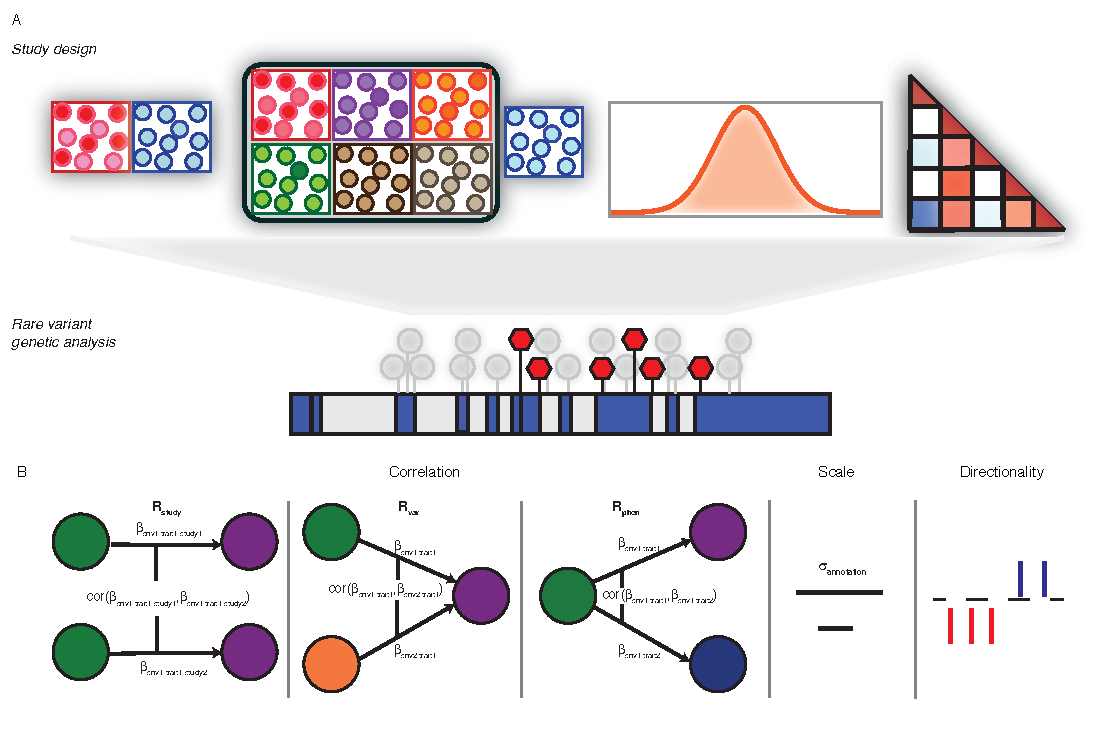
\includegraphics[width=\textwidth]{../figures/final/Figure_01.pdf}
\caption{{\bf Schematic overview of MRP.}}
%\paragraph*{Fig 1. Schematic overview of MRP.}
\label{overview}
A: MRP is suitable for a broad range of rare variant association study designs including (from left to right): i) case-control, ii) multiple diseases with shared controls, iii) single quantitative phenotype, and iv) mixture of case-control and quantitative phenotypes. B: Diagram of factors considered in rare variant association analysis including the correlation matrices: $\mathbf{R_{\textrm{study}}}$  (expected correlation of genetic effects among a group of studies), $\mathbf{R_{\textrm{var}}}$ (expected correlation of genetic effects among a group of variants), and $\mathbf{R_{\textrm{phen}}}$ (expected correlation of genetic effects among a group of phenotypes); the scale parameter for genetic variant annotation; and the location of genetic effects, which may be used to prioritize or identify protective modifiers of disease risk.
\end{figure}

\begin{figure}[!h]
%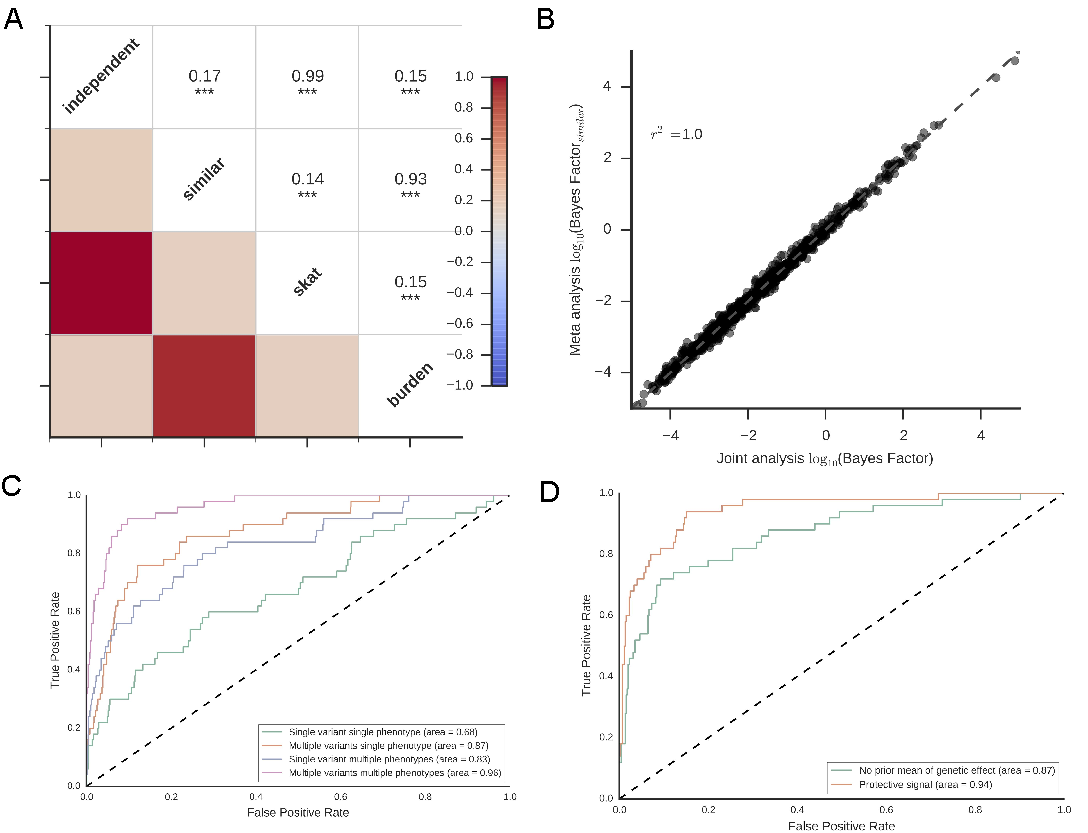
\includegraphics[width=\textwidth]{../figures/final/Figure_02.pdf}
\caption{{\bf Simulation studies.}}
\label{simresults}
A: Comparison of $-\log_{10}$(p-values) from frequentist $\textrm{BF}_{\textrm{MRP}}$ approximation for an independent effects and a similar effects model to commonly used gene-based statistical tests (skat and burden). B: Comparison of log10(Bayes Factors) obtained when raw genotype and phenotype data is available to a scenario where summary statistics only was available and similar effects across studies is assumed. C: From single variant and single phenotype to multiple variants and multiple phenotypes gene discovery: ROC curves for detecting gene association to any of the phenotypes using single variant/single phenotype association (green) to multiple variants and multiple phenotypes association (purple). D: ROC curves for detecting gene association when incorporating prior mean of genetic effects (orange) to identify protective alleles.
\end{figure}

%% FIGURE: ASTHMA MANHATTAN AND FOREST FOR BMA
\begin{figure}[!h]
%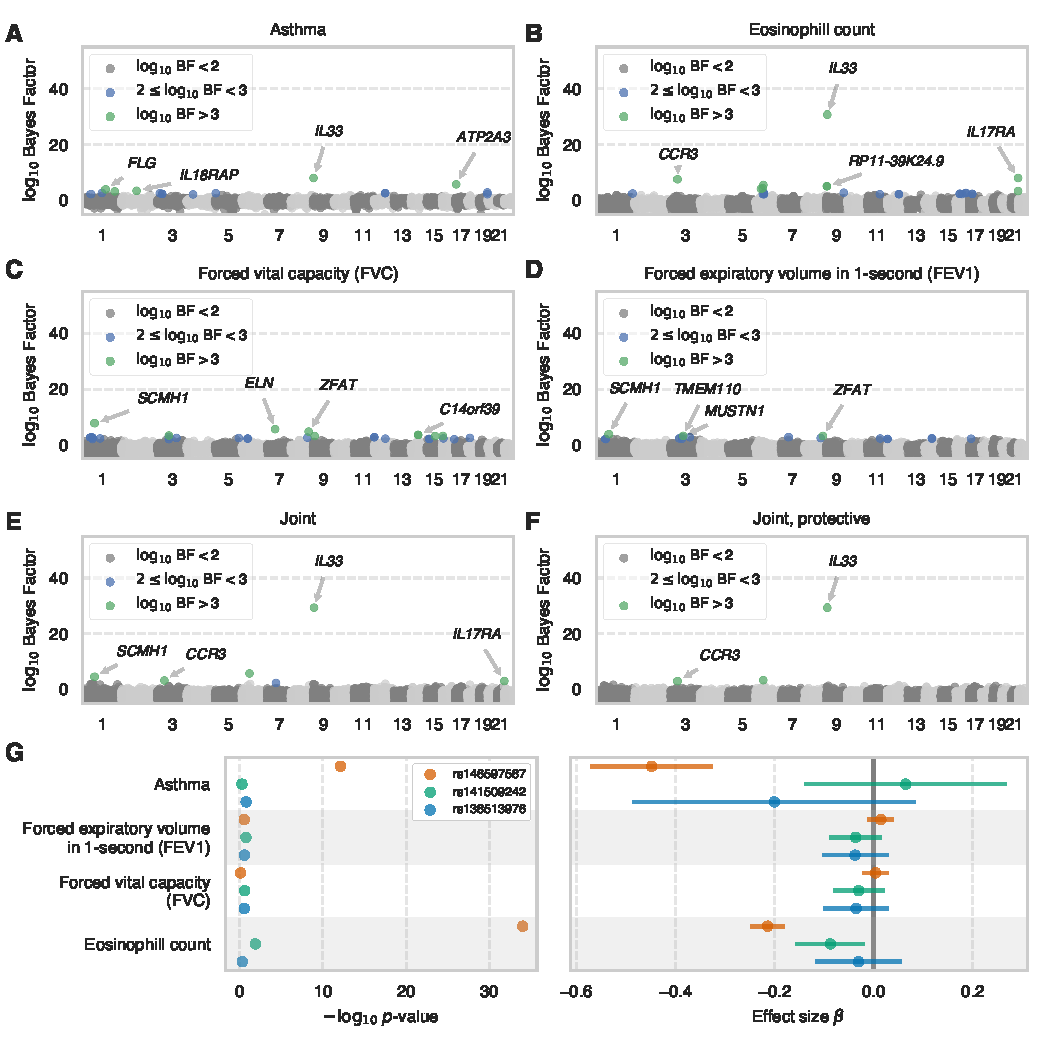
\includegraphics[width=\textwidth]{../figures/final/Figure_03.pdf}
\caption{{\bf Results for asthma application.}}
\label{asthma_bma}
$\log_{10}$ Bayes Factors from applying MRP and Bayesian model averaging to summary statistics for missense and protein-truncating variants from (A) asthma (HC382), (B) eosinophil counts (INI30150), (C) forced vital capacity (FVC, INI3062), (D) forced expiratory volume in 1-second (FEV$_1$, INI3063), (E) all four traits jointly, and (F) all four traits jointly with focus on protective effects. The four genes outside of chromosome 6 with the largest Bayes Factors greater than three are labeled in each plot. Only $\log_{10}$ Bayes Factors greater than -5 are plotted. (F) $-\log_{10}$ $p$-values (left panel) and estimated effect sizes with 95\% confidence intervals (right panel) for missense variants and PTVs in \textit{IL33} for each phenotype
\end{figure}

\begin{figure}[!h]
%%\in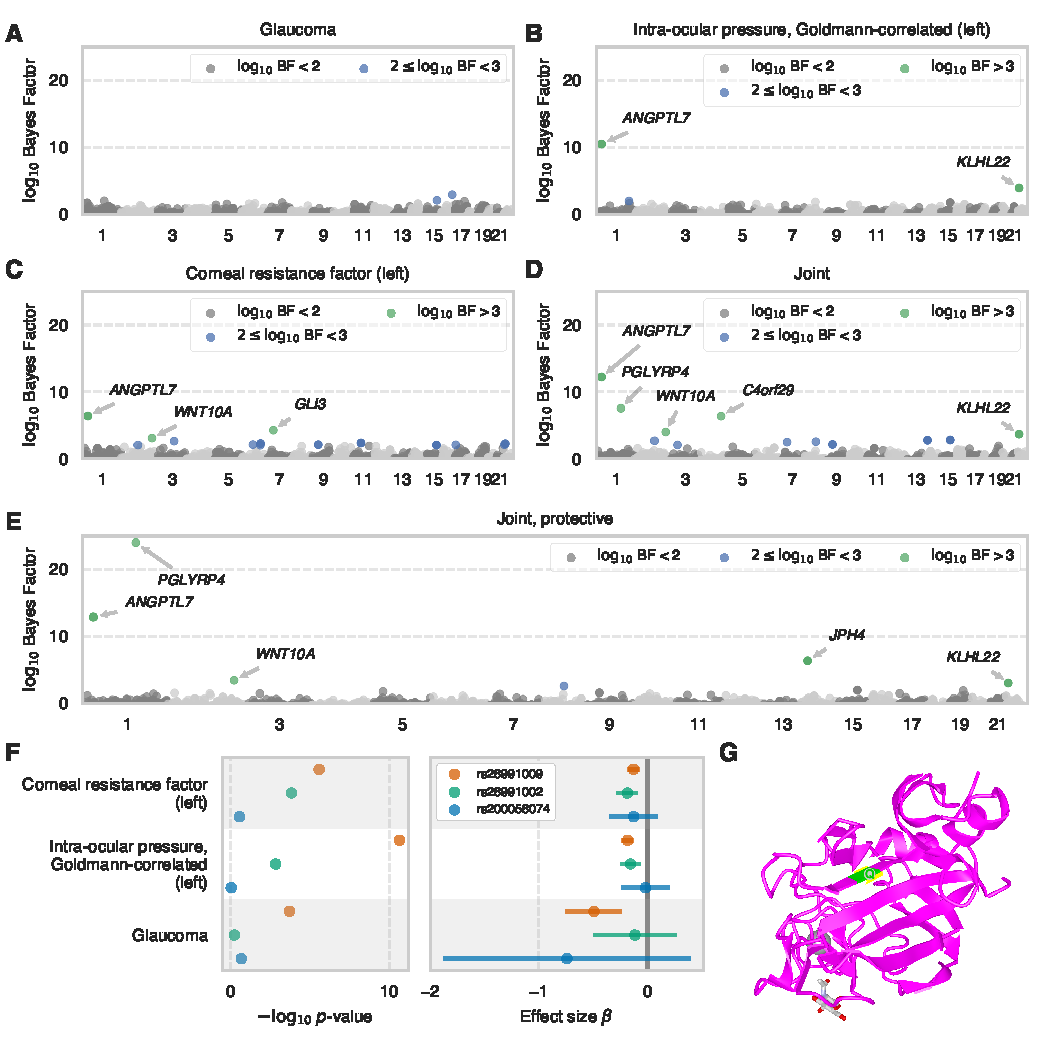
\includegraphics[width=\textwidth]{../figures/final/Figure_04.pdf}
\caption{{\bf Results for glaucoma application.}}
\label{glaucoma_bma}
$\log_{10}$ Bayes Factors from applying MRP and Bayesian model averaging to summary statistics for missense and protein-truncating variants from (A) glaucoma (HC276), (B) intra-ocular pressure (INI5263), (C) corneal resistance factor (INI5265), and (D) all three traits jointly. (E) shows the results of a joint analysis focused on finding rare variants that protect against glaucoma. The genes outside of chromosome 6 with with Bayes Factor greater than three are indicated by arrows. Only $\log_{10}$ Bayes Factors greater than zero are plotted. F: $-\log_{10}$ $p$-values (left panel) and estimated effect sizes with 95\% confidence intervals (right panel) for missense variants and PTVs in \textit{ANGPTL7} for all three phenotypes. G: Location of rs28991009 variant (green, p.Q175H, NM\_021146) for the protein 1JC9\_A homologous to \textit{ANGPTL7}.
\end{figure}

\pagebreak

\section*{Supporting Information Legends}

% Include only the SI item label in the paragraph heading. Use the \nameref{label} command to cite SI items in the text.

\paragraph*{S1 Appendix.}
\label{S1_Appendix}
{\bf MRP model details.} Specification of the MRP model including the likelihood function, priors, and Bayes factor calculation.

%\begin{figure}[H]
%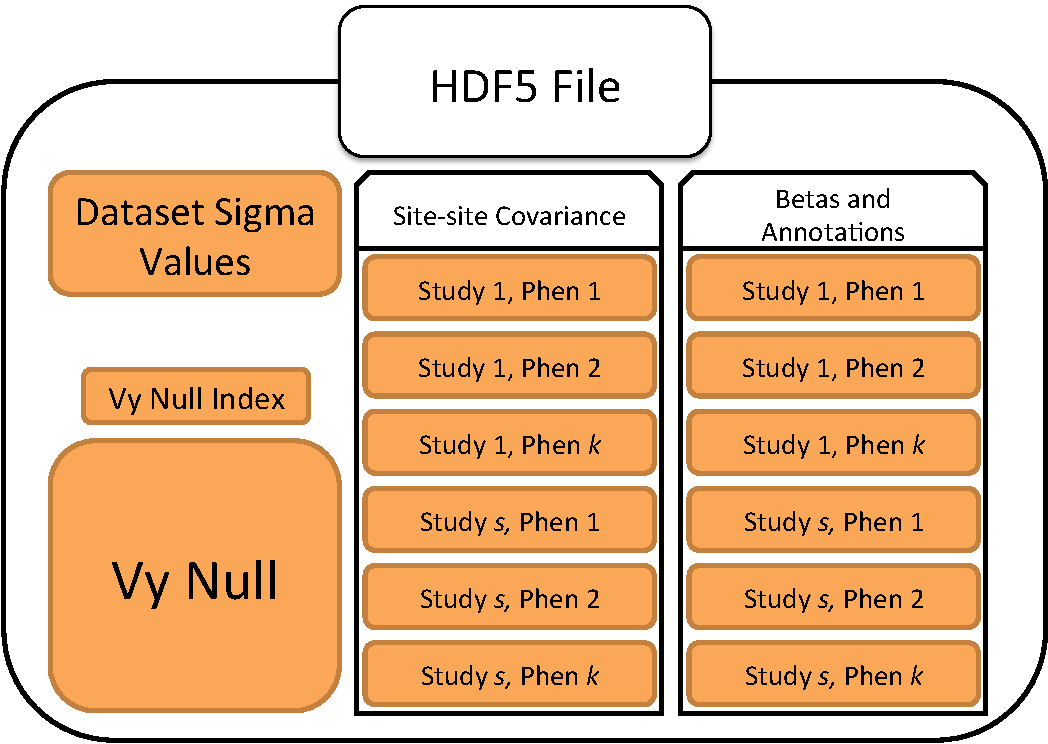
\includegraphics[width=\textwidth]{../figures/final/Figure_S01.pdf}
%\end{figure}
\paragraph*{S1 Fig.}
\label{hdf5_fig}
{\bf HDF5 Implementation.} Our HDF5 implementation contained the following components: first, a group with one table per annotation file. All effect size (beta) values and study-specific annotations were contained here, and the number of tables is limited by $S\ \textrm{(the number of studies)} \times K\ \textrm{(the number of traits)}$. Second, a group with site-site covariance data. While these covariance matrices may have dimension $M\ \textrm{(the number of variants)} \times M$, we store the data as tables, each row specifiying the covariance between two variants. The number of tables should be the same as the previous set, capped by $S\ \textrm{(the number of studies)} \times K\ \textrm{(the number of traits)}$. Third, we store one table with sigma values for each study/phenotype combination. In the event that the traits were rank-normal transformation was performed these sigma values are equal to 1. These are used to compute correlation between two datasets. Finally, we store a matrix/table pair for Vy null and its index. The Vy null matrix has dimensions $ (S \times K) \times (S \times K)$ each entry specifying the estimated correlation of effect sizes between two datasets. The index table encodes row/column position of each dataset.

%\begin{figure}[H]
%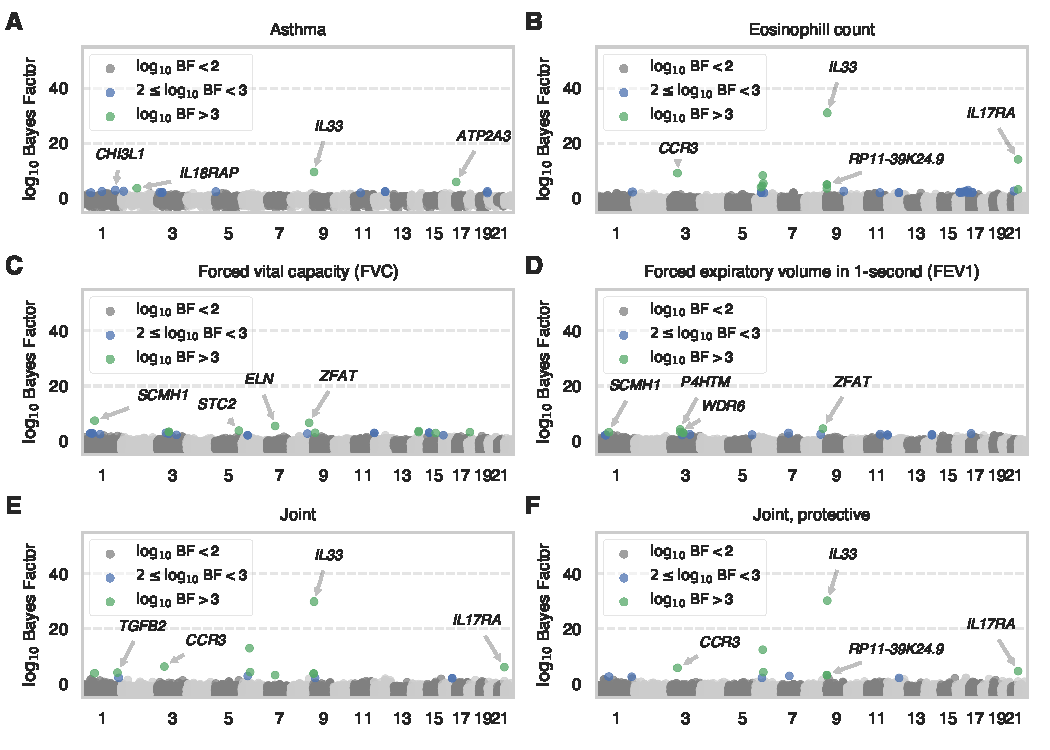
\includegraphics[width=\textwidth]{../figures/final/Figure_S02.pdf}
%\end{figure}
\paragraph*{S2 Fig.}
\label{gcorr_fig}
{\bf Genetic correlations.} Genetic correlations for (A) asthma and related phenotypes and (B) glaucoma and related phenotypes estimated using MVPMM. Genetic correlations for (C) asthma and related phenotypes and (D) glaucoma and related phenotypes estimated using LD score regression.

%% FIGURE: ASTHMA MANHATTAN AND FOREST FOR INDEPENDENT EFFECTS
%\begin{figure}[H]
%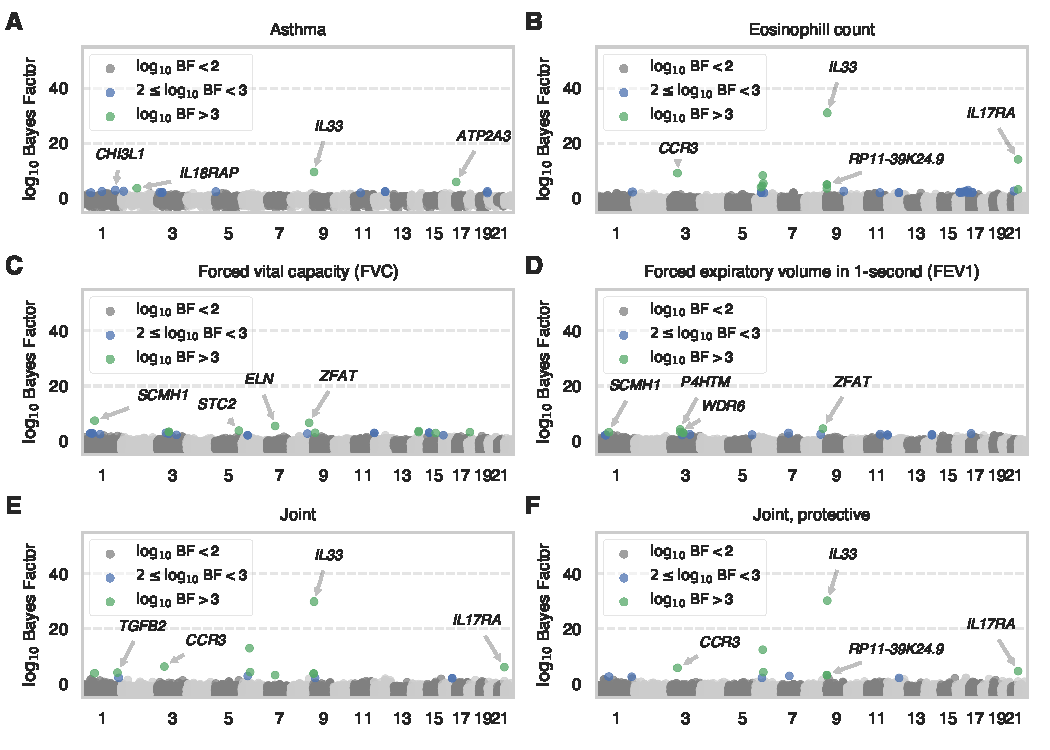
\includegraphics[width=\textwidth]{../figures/final/Figure_S03.pdf}
%\end{figure}
\paragraph*{S3 Fig.}
\label{asthma_independent}
{\bf Results for independent effects model applied to asthma, eosinophil counts, FEV$_1$, and FVC.} $\log_{10}$ Bayes Factors from applying MRP independent effects model to summary statistics for missense and protein-truncating variants from (A) asthma (HC382), (B) eosinophil counts (INI30150), (C) forced vital capacity (FVC, INI3062), (D) forced expiratory volume in 1-second (FEV$_1$, INI3063), (E) all four traits jointly, and (F) all four traits jointly with focus on protective effects. The four genes outside of chromosome 6 with the largest Bayes Factors greater than three are labeled in each plot. Only $\log_{10}$ Bayes Factors greater than -5 are plotted.

%% FIGURE: ASTHMA MANHATTAN AND FOREST FOR SIMILAR EFFECTS
%\begin{figure}[H]
%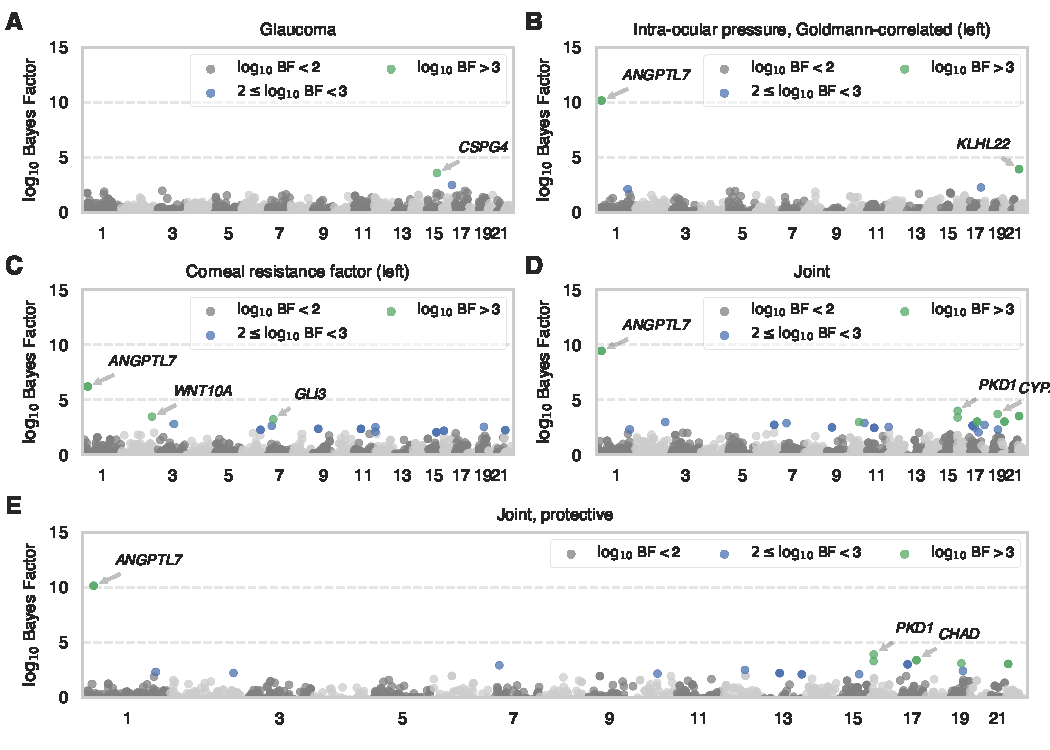
\includegraphics[width=\textwidth]{../figures/final/Figure_S04.pdf}
%\end{figure}
\paragraph*{S4 Fig.}
\label{asthma_similar}
{\bf Results for similar effects model applied to asthma, eosinophil counts, FEV$_1$, and FVC.} $\log_{10}$ Bayes Factors from applying MRP similar effects model to summary statistics for missense and protein-truncating variants from (A) asthma (HC382), (B) eosinophil counts (INI30150), (C) forced vital capacity (FVC, INI3062), (D) forced expiratory volume in 1-second (FEV$_1$, INI3063), (E) all four traits jointly, and (F) all four traits jointly with focus on protective effects. The four genes outside of chromosome 6 with the largest Bayes Factors greater than three are labeled in each plot. Only $\log_{10}$ Bayes Factors greater than -5 are plotted.

%\begin{figure}[H]
%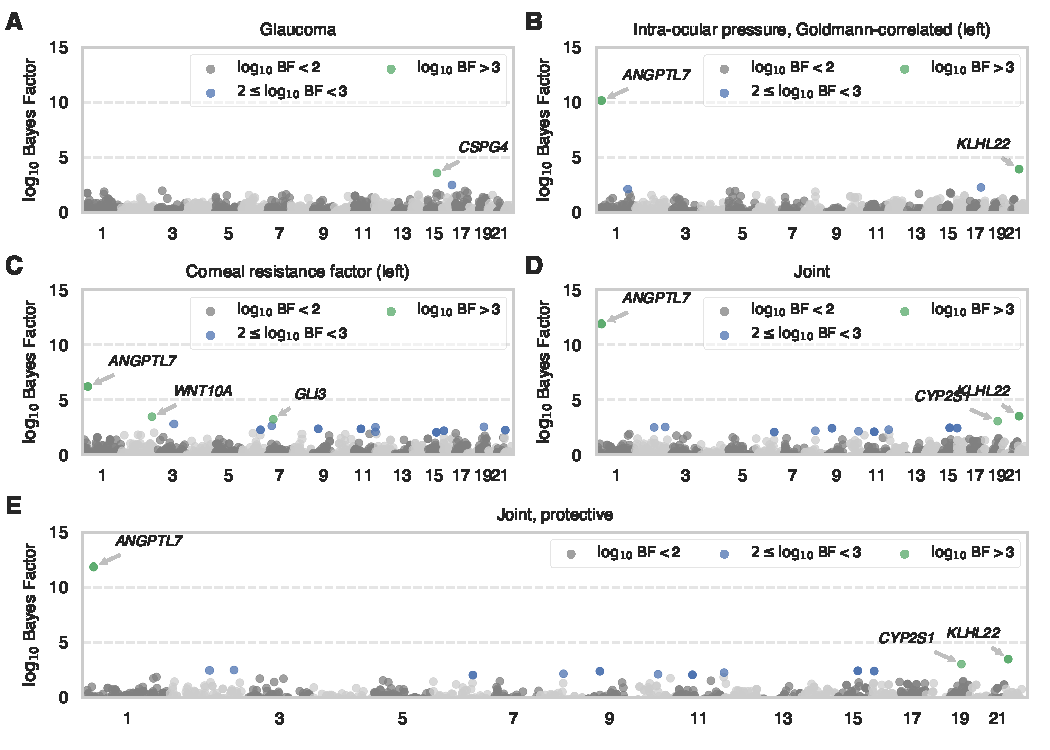
\includegraphics[width=\textwidth]{../figures/final/Figure_S05.pdf}
%\end{figure}
\paragraph*{S5 Fig.}
\label{glaucoma_independent}
{\bf Results for independent effects model applied to glaucoma intra-ocular pressure, and corneal resistance factor.} $\log_{10}$ Bayes Factors from applying MRP independent effects model to summary statistics for missense and protein-truncating variants from (A) glaucoma (HC276), (B) intra-ocular pressure (INI5263), (C) corneal resistance factor (INI5265), and (D) all three traits jointly. (E) shows the results of a joint analysis focused on finding rare variants that protect against glaucoma. The genes outside of chromosome 6 with with Bayes Factor greater than three are indicated by arrows. Only $\log_{10}$ Bayes Factors greater than zero are plotted.

%\begin{figure}[H]
%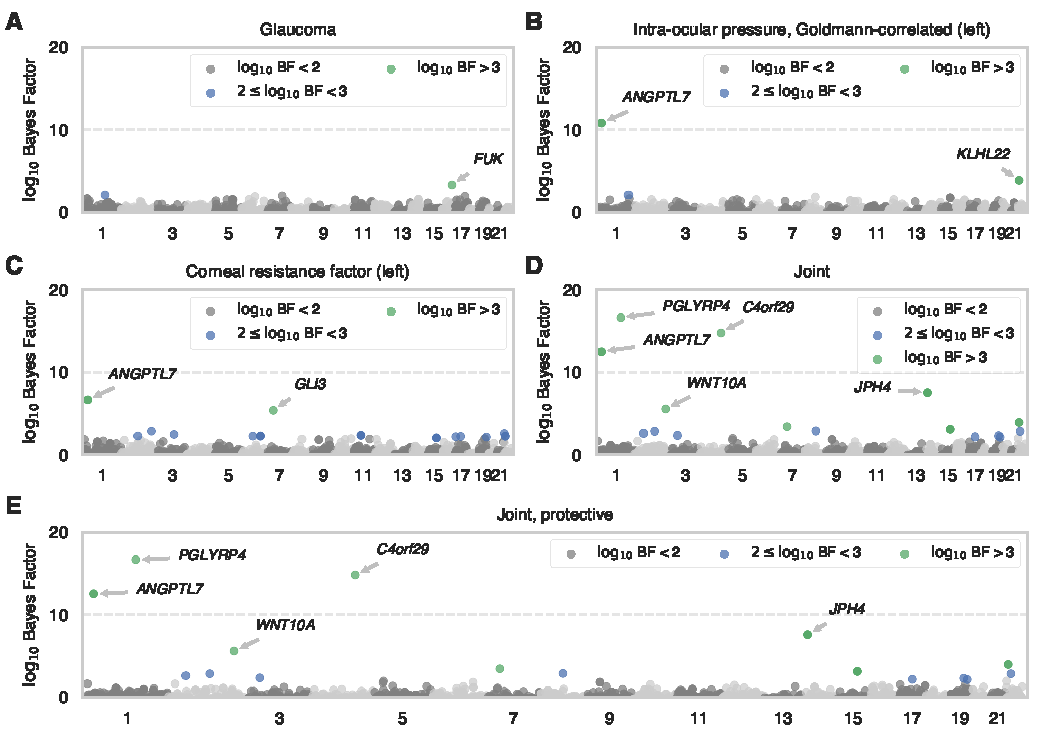
\includegraphics[width=\textwidth]{../figures/final/Figure_S06.pdf}
%\end{figure}
\paragraph*{S6 Fig.}
\label{glaucoma_similar}
{\bf Results for similar effects model applied to glaucoma intra-ocular pressure, and corneal resistance factor.} $\log_{10}$ Bayes Factors from applying MRP similar effects model to summary statistics for missense and protein-truncating variants from (A) glaucoma (HC276), (B) intra-ocular pressure (INI5263), (C) corneal resistance factor (INI5265), and (D) all three traits jointly. (E) shows the results of a joint analysis focused on finding rare variants that protect against glaucoma. The genes outside of chromosome 6 with with Bayes Factor greater than three are indicated by arrows. Only $\log_{10}$ Bayes Factors greater than zero are plotted.

\pagebreak

\section*{Tables}

\begin{table}[!ht]
\begin{adjustwidth}{-2.25in}{0in} % Comment out/remove adjustwidth environment if table fits in text column.
\centering
%\caption{
%{\bf $\log_{10}$ Bayes Factors for genes highlighted in Figure~\ref{asthma_bma}.}}
\begin{tabular}{|l+l|l|l|l|l|l|}
\hline
{\bf Gene} & {\bf Joint, protective} & {\bf Joint} & {\bf Eosinophil count} & {\bf FVC} & {\bf FEV$_1$} & {\bf Asthma} \\
\thickhline
\textit{IL33}         &              29.4 &   29.3 &             30.6 &  -2.3 &  -2.2 &    8.1 \\
\hline
\textit{CCR3}         &               3.1 &    3.3 &              7.4 &  -1.4 &  -1.6 &   -0.5 \\
\hline
\textit{RP11-39K24.9} &               0.8 &    1.8 &              4.9 &  -0.1 &  -0.4 &    0.3 \\
\hline
\textit{SCMH1}        &               0.5 &    4.7 &             -1.5 &   7.7 &   3.8 &   -0.7 \\
\hline
\textit{MUSTN1}       &               0.4 &    1.1 &             -1.2 &   2.9 &   2.9 &   -0.6 \\
\hline
\textit{ZFAT}         &               0.3 &    1.3 &             -2.0 &   4.7 &   3.1 &   -0.4 \\
\hline
\textit{ELN}          &               0.2 &    2.5 &             -1.0 &   5.6 &   2.9 &   -0.6 \\
\hline
\textit{C14orf39}     &              -0.7 &   -0.0 &             -1.1 &   3.5 &   2.5 &    0.0 \\
\hline
\textit{TMEM110}      &              -0.9 &    1.1 &             -1.0 &   3.3 &   3.1 &   -0.6 \\
\hline
\textit{IL17RA}       &              -4.4 &    3.1 &              7.9 &  -2.7 &  -2.5 &   -1.1 \\
\hline
\textit{IL18RAP}      &              -9.6 &   -0.9 &             -1.0 &  -1.6 &  -1.7 &    3.5 \\
\hline
\textit{ATP2A3}       &             \textendash11.9 &   -0.8 &             -1.2 &  -2.1 &  -2.2 &    5.8 \\
\hline
\textit{FLG}          &             -20.1 &  -17.2 &             -6.0 &  -7.4 &  -8.5 &    4.0 \\
\hline
\end{tabular}
\label{asthma_table}
\end{adjustwidth}
\end{table}
\paragraph*{S1 Table.}
\label{asthma_table}
{\bf Highlighted genes from asthma analysis.} $\log_{10}$ Bayes Factors for genes highlighted in Figure~\ref{asthma_bma}.


% %% TABLE: GLAUCOMA GENES OF INTEREST
\begin{table}[!ht]
\begin{adjustwidth}{-2.25in}{0in} % Comment out/remove adjustwidth environment if table fits in text column.
\centering
%\caption{
%{\bf $\log_{10}$ Bayes Factors for genes highlighted in Figure~\ref{glaucoma_bma}.}}
\begin{tabular}{|l+p{3cm}|p{1cm}|p{1.6cm}|p{3.8cm}|p{3.4cm}|}
\hline
{\bf Gene} & {\bf Joint, protective} & {\bf Joint} & {\bf Glaucoma} & {\bf Intra-ocular pressure, Goldmann-correlated} & {\bf Corneal resistance factor} \\
\thickhline
\textit{ANGPTL7} &              13.1 &  12.2 &      1.7 &                                       10.5 &                       6.4 \\
\hline
\textit{KLHL22}  &               3.1 &   3.7 &     -0.2 &                                        3.9 &                       2.2 \\
\hline
\textit{WNT10A}  &               2.6 &   2.6 &     -0.2 &                                       -0.6 &                       3.1 \\
\hline
\textit{GLI3}    &               0.5 &   2.3 &     -0.4 &                                       -0.1 &                       4.3 \\
\hline
\end{tabular}
\end{adjustwidth}
\end{table}
\paragraph*{S2 Table.}
\label{glaucoma_table}
{\bf Highlighted genes from glaucoma analysis.} $\log_{10}$ Bayes Factors for genes highlighted in Figure~\ref{glaucoma_bma}.


\end{document}
